\documentclass[5p,sort&compress]{elsarticle}

\usepackage{amssymb}    % Mathematical symbols
\usepackage{amsmath}    % More options for mathematics
\usepackage{subfigure}  % More options for figures
\usepackage{epstopdf}   % Convert eps to pdf
\usepackage[separate-uncertainty=true]{siunitx}   % Proper formatting of units in math mode
\usepackage{color}      % Supports text color if needed
\usepackage{soul}       % https://ctan.org/pkg/soul
\usepackage{lmodern}    % Loading fonts
\usepackage{hyperref}   % To insert clickable references/urls
\usepackage{listings}   % To input code in the text
\usepackage{amsmath}
\usepackage{amsmath}
\usepackage{amssymb}
\usepackage{graphicx}
\usepackage{epstopdf}
\usepackage{booktabs}
\setlength{\parskip}{2em}
\newcommand{\stirlingii}{\genfrac{\{}{\}}{0pt}{}}

% Choose the style of the reference list (do not change)
\bibliographystyle{elsarticle-num}

\journal{ifding/learning-notes}

% Begin the document

\begin{document}

\begin{frontmatter}
    \title{Ch 8: Graphical Models}
    \author{ifding}
    
    \begin{abstract}
        Bayesian Networks, Conditional Independence, Inference in Graphical Models
    \end{abstract}


\end{frontmatter}

%% How to make a heading and divide the documents into different sections

All of the probabilistic inference and learning manipulations, no matter how complex, amount to repeated application of two equations: the sum rule and the product rule. 

In a \textit{probabilistic graphical model}, each node represents a random variable (or group of random variables), and the edges express probabilistic relationships between these variables. \textit{Bayesian networks} are known as directed graphical models, and \textit{Markov random fields} are known as undirected graphical models. Directed graphs are useful for expressing causal relationships between random variables, whereas undirected graphs are better suited to expressing soft constraints between random variables.


\section{Bayesian Networks}

Consider an arbitrary joint distribution $p(a, b, c)$ over three variables a, b and c.
\begin{equation}
p(a, b, c) = p(c | a, b) p(a,b) = p(c | a, b) p(b | a) p(a)
\end{equation}

\begin{figure}[ht]
     \centering
     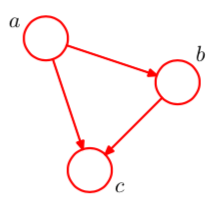
\includegraphics[width = 0.5\linewidth]{figure/figure8_1.png}
     \caption{A directed graphical model.}
     \label{fig:8_1}
\end{figure}

As shown in Figure~\ref{fig:8_1}, if there is a link going from a node $a$ to a node $b$, then we say that node $a$ is the \textit{parent} of node $b$, and we say that node $b$ is the \textit{child} of node $a$. For a graph with $K$ nodes, the joint distribution is given by
\begin{equation}
p(\mathbf{x})=\prod_{k=1}^{K} p\left(x_{k} | \mathrm{pa}_{k}\right)
\end{equation}
where $pa_k$ denotes the set of parents of $x_k$, and $\mathbf{x} = \{x_1, \ldots, x_K\}$. This key equation expresses the \textit{factorization} properties of joint distribution for directed graphical model.


\subsection{Example: Polynomial regression}

Consider the Bayesian polynomial regression model, the random variables are the vector of polynomial coefficients $\mathbf{w}$ and the observed data $\mathbf{t} = (t_1, \ldots, t_N)^{\mathrm{T}}$, the noise variance $\sigma^2$, and the hyperparameter $\alpha$ representing the precision of the Gaussian prior over $\mathbf{w}$. The joint distribution is given by the product of the prior $p(\mathbf{w})$ and N conditional distributions $p(t_n|\mathbf{w})$ for $n = 1, \ldots, N$
\begin{equation}
p(\mathbf{t}, \mathbf{w})=p(\mathbf{w}) \prod_{n=1}^{N} p\left(t_{n} | \mathbf{w}\right)
\end{equation}

\begin{figure}[ht]
     \centering
     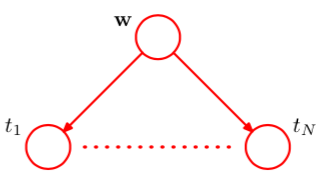
\includegraphics[width = 0.5\linewidth]{figure/figure8_3.png}
     \caption{Directed graphical model representing the joint distribution corresponding to the Bayesian polynomial regression model.}
     \label{fig:8_3}
\end{figure}

We shall find it helpful to make the parameters of a model, as well as its stochastic variables, explicit.
\begin{equation}
p\left(\mathbf{t}, \mathbf{w} | \mathbf{x}, \alpha, \sigma^{2}\right)=p(\mathbf{w} | \alpha) \prod_{n=1}^{N} p\left(t_{n} | \mathbf{w}, x_{n}, \sigma^{2}\right)
\end{equation}

We can make $\mathbf{x}$ and $\alpha$ explicit in the graphical representation. Random variables will be denoted by option circles, and deterministic parameters will be denoted by smaller solid circles. A \textit{plate} (the box labelled N) is introduced to represent N nodes of which only a single example $t_n$ is shown explicitly.

\begin{figure}[ht]
     \centering
     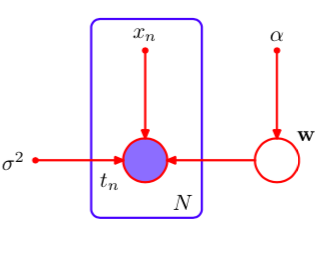
\includegraphics[width = 0.6\linewidth]{figure/figure8_6.png}
     \caption{The deterministic parameters shown explicitly by the smaller solid nodes, observed variables $\{t_n\}$ are denoted by shading the corresponding nodes, the value of $\mathbf{w}$ is not observed, and so $\mathbf{w}$ is an example of a \textit{latent} variable.}
     \label{fig:8_6}
\end{figure}


\subsection{Discrete variables}

The probability distribution $p(\mathbf{x}| \boldsymbol{\mu})$ for a single discrete variable $\mathbf{x}$ having K possible states (using the 1-of-K representation) is given by
\begin{equation}
p(\mathbf{x} | \boldsymbol{\mu})=\prod_{k=1}^{K} \mu_{k}^{x_{k}}  
\end{equation}
and is governed by the parameters $\boldsymbol{\mu} = (\mu_1, \ldots, \mu_K)^{\mathrm{T}}$. Due to the constraint $\sum_{k} \mu_{k}=1$, only $K-1$ values for $\mu_k$ need to be specified in order to define the distribution.


\section{Conditional Independence}

Consider three variables $a$, $b$ and $c$,
\begin{equation}
p(a | b, c)=p(a | c)
\end{equation}
We say that $a$ is conditionally independent of $b$ given $c$. 
\begin{equation}
\begin{aligned} p(a, b | c) &=p(a | b, c) p(b | c) \\ &=p(a | c) p(b | c) \end{aligned}
\end{equation}
The variables $a$ and $b$ are statistically independent, given $c$. Conditional independence properties play an important role in using probabilistic by simplifying both the structure of a model ans the computations needed to perform inference and learning under that model.

\subsection{Three example graphs}

The first of the three examples:
\begin{equation}
    p(a,b,c) = p(a|c) p(b|c) p(c)
\end{equation}
If none of the variables are observed, then we can investigate whether $a$ and $b$ are independent by marginalizing both sides with respect to c
\begin{equation}
p(a, b)=\sum_{c} p(a | c) p(b | c) p(c)
\end{equation}
Now suppose we condition on the variable $c$, as represented by the graph of Figure~\ref{fig:8_16}, the conditional distribution of $a$ and $b$, given $c$, can be written in the form
\begin{equation}
\begin{aligned} p(a, b | c) &=\frac{p(a, b, c)}{p(c)} \\ &=p(a | c) p(b | c) \end{aligned}
\end{equation}


\begin{figure}[ht]
     \centering
     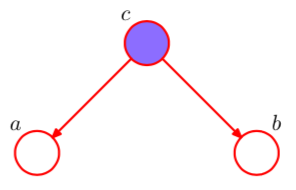
\includegraphics[width = 0.6\linewidth]{figure/figure8_16.png}
     \caption{The variables $a$ and $b$ of conditional independence on the value of variable $c$.}
     \label{fig:8_16}
\end{figure}

The second example is shown in Figure~\ref{fig:8_18}.
\begin{equation}
p(a, b, c)=p(a) p(c | a) p(b | c)
\end{equation}
First of all, suppose that none of the variables are observed. Again, we can test to see if $a$ and $b$ are independent by marginalizing over $c$ to give
\begin{equation}
p(a, b)=p(a) \sum_{c} p(c | a) p(b | c)=p(a) p(b | a)
\end{equation}


\begin{figure}[ht]
     \centering
     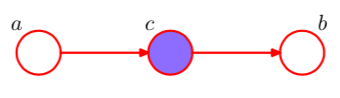
\includegraphics[width =0.6\linewidth]{figure/figure8_18.png}
     \caption{3-node graphs conditioning on node $c$.}
     \label{fig:8_18}
\end{figure}

Now suppose we condition on node $c$, as shown in Figure~\ref{fig:8_18}. Using Bayes' theorem,
\begin{equation}
\begin{aligned} p(a, b | c) &=\frac{p(a, b, c)}{p(c)} \\ &=\frac{p(a) p(c | a) p(b | c)}{p(c)} \\ &=p(a | c) p(b | c) \end{aligned}
\end{equation}

Finally, we consider the third of our 3-node examples, shown by the graph in Figure~\ref{fig:8_20}. The joint distribution can again be written down
\begin{equation}
p(a, b, c)=p(a) p(b) p(c | a, b)
\end{equation}
Consider first the case where none of the variables are observed. Marginalizing both sides over $c$
\begin{equation}
p(a, b)=p(a) p(b)
\end{equation}
and so $a$ and $b$ are independent with no variables observed. The conditional distribution of $a$ and $b$ is then given by
\begin{equation}
\begin{aligned} p(a, b | c) &=\frac{p(a, b, c)}{p(c)} \\ &=\frac{p(a) p(b) p(c | a, b)}{p(c)} \end{aligned}
\end{equation}
which in general does not factorize into the product $p(a)p(b)$.


\begin{figure}[ht]
     \centering
     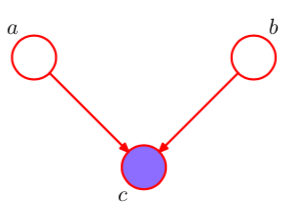
\includegraphics[width =0.6\linewidth]{figure/figure8_20.png}
     \caption{3-node graphs conditioning on node $c$. The act of conditioning induces a dependence between $a$ and $b$.}
     \label{fig:8_20}
\end{figure}

It's worth spending a moment to understand further the unusual behaviour of the graph of Figure~\ref{fig:8_20}. Consider a particular instance of such a graph corresponding to a problem with three binary random variables relating to the fuel system on a car, as shown in Figure~\ref{fig:8_21}.

\begin{figure}[ht]
     \centering
     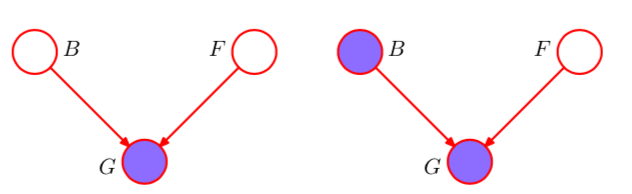
\includegraphics[width =\linewidth]{figure/figure8_21.png}
     \caption{The three nodes represent the state of the battery(B), the state of the fuel tank (F) and the reading on the electric fuel gauge (G).}
     \label{fig:8_21}
\end{figure}

The B variables represent the state of a battery that is either charged (B=1) or flat (B=0), F represent the state of the fuel tank that is either full (F=1) or empty (F=0), and G indicates either full (G=1) or empty (G=0). The prior probabilities
\begin{equation}
    p(B=1) = 0.9, ~
    p(F=1) = 0.9
\end{equation}

Given B and F, the G reads full with probabilities given by
\begin{equation}
\begin{array}{l}{p(G=1 | B=1, F=1)=0.8} \\ {p(G=1 | B=1, F=0)=0.2} \\ {p(G=1 | B=0, F=1)=0.2} \\ {p(G=1 | B=0, F=0)=0.1}\end{array}
\end{equation}

The prior probability of  fuel tank being empty is $p(F=0) = 1 - 0.9 = 0.1$. Now suppose that we observe the fuel gauge and discover that it reads empty, i.e., $G=0$, corresponding to the left-hand graph in Figure~\ref{fig:8_21}.
\begin{equation}
\begin{aligned}
p(G=0)=\sum_{B \in\{0,1\}} \sum_{F \in\{0,1\}} p(G=0 | B, F) p(B) p(F) \\
= (1-0.8)*0.9*0.9 + (1-0.2)*0.9*(1-0.9) + \\
(1-0.2)*(1-0.9)*0.9 + (1-0.1)*(1-0.9)*(1-0.9) \\
=0.315
\end{aligned}
\end{equation}
and similarly we evaluate
\begin{equation}
p(G=0 | F=0)=\sum_{B \in\{0,1\}} p(G=0 | B, F=0) p(B)=0.81
\end{equation}
and using these results we have
\begin{equation}
p(F=0 | G=0)=\frac{p(G=0 | F=0) p(F=0)}{p(G=0)} \simeq 0.257
\end{equation}
and so $p(F=0|G=0) > p(F=0)$. Thus observing that the gauge reads empty makes it more likely that the tank is indeed empty.

We have now observed the states of the battery and find that it is flat, i.e., $B=0$. We have now observed the states of both the fuel gauge and the battery, as shown by the right-hand graph in Figure~\ref{fig:8_21}.
\begin{equation}
\begin{aligned}
p(F=0 | G=0, B=0) \\
= \frac{p(G=0 | B=0, F=0) p(F=0) p(B=0)}{\sum_{F \in\{0,1\}} p(G=0 | B=0, F) p(F) p(B=0)} \\
= \frac{p(G=0 | B=0, F=0) p(F=0)}{\sum_{F \in\{0,1\}} p(G=0 | B=0, F) p(F)} \simeq 0.111
\end{aligned}
\end{equation}
Thus the probability that the tank is empty has decreased (from 0.257 to 0.111) as a result of the observation of the state of the battery.


\section{Inference in Graphical Models}

To start with, let us consider the graphical interpretation of the joint distribution $p(x,y) = p(x)p(y|x)$. This can be represented by the directed graph shown in Figure~\ref{fig:8_37}(a). Now suppose we observe the value of $y$, as indicated by the shaded node in Figure~\ref{fig:8_37}(b).

\begin{figure}[ht]
     \centering
     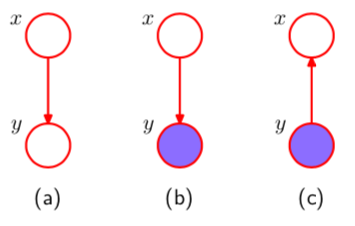
\includegraphics[width =0.9\linewidth]{figure/figure8_37.png}
     \caption{A graphical representation of Bayes' theorem.}
     \label{fig:8_37}
\end{figure}

We can view the marginal distribution $p(x)$ as a prior over the latent variable $x$, and our goal is to infer the corresponding posterior distribution over $x$.
\begin{equation}
p(y)=\sum_{x^{\prime}} p\left(y | x^{\prime}\right) p\left(x^{\prime}\right)
\end{equation}
which can then be used in Bayes' theorem to calculate
\begin{equation}
p(x | y)=\frac{p(y | x) p(x)}{p(y)}
\end{equation}
The direction of the arrow is reversed, as shown in Figure~\ref{fig:8_37}(c).





%\section*{References}
\bibliography{references}

\begin{thebibliography}{9}

\bibitem{Bishop} 
Bishop, Christopher M. Pattern recognition and machine learning. springer, 2006.


\end{thebibliography}
\end{document}